\section*{Đề thi thử THPTQG Sở GD\&ĐT Cà Mau 25--26, Lần 1}

\caulc
\Opensolutionfile{ans}[ans/ans-26-2-CaMau-SoGD-L1-LC]
%%==========Câu 1
\begin{ex}%[40-26-2-CaMau-SoGD-L1]%[Doan Thinh,26-2-DuAnDeTHPT2025-2026]%[1D2N3-4]
	Cho cấp số nhân $(u_n)$ có số hạng đầu $u_1=2$ và công bội $ q=-2$. Giá trị $u_5$ là
	\choice
	{ $-32$}
	{\True $32$}
	{ $-16$}
	{ $-6$}
	\loigiai{
		$$u_5=u_1\cdot q^4=2\cdot(-2)^4=32.$$
	}
\end{ex}
%%==========Câu 2
\begin{ex}%[40-26-2-CaMau-SoGD-L1]%[Doan Thinh,26-2-DuAnDeTHPT2025-2026]%[2D4H3-4]
	Xét một vật thể giới hạn bởi hai mặt phẳng $ x=0$; $x=3$. Biết rằng khi cắt vật thể bởi mặt phẳng vuông góc với trục $Ox$ tại điểm có hoành độ $x$, $\left(0\le x\le 3\right)$ ta được mặt cắt là một hình vuông có độ dài cạnh bằng $\sqrt{9-x^2}$. Thể tích của vật thể đó bằng
	\choice
	{\True $18$}
	{ $36$}
	{ $36\pi $}
	{ $18\pi $}
	\loigiai{
		Thể tích của vật thể là $V =\displaystyle\int_0^3 (9-x^2)dx = 18$.
	}
\end{ex}
%%==========Câu 3
\begin{ex}%[40-26-2-CaMau-SoGD-L1]%[Doan Thinh,26-2-DuAnDeTHPT2025-2026]%[1D6H4-4]
	Cho phương trình $\log_2(x^2+x+1)=3$ có hai nghiệm $x_1$, $x_2$. Khi đó $x_1\cdot x_2$ bằng
	\choice
	{\True $-7$}
	{ $7$}
	{ $-1$}
	{ $1$}
	\loigiai{
		$\log_2(x^2+x+1)=3\Leftrightarrow x^2+x+1=2^3\Leftrightarrow x^2+x-7=0$.\\
		Suy ra $x_1\cdot x_2=\dfrac{-7}{1}=-7$. 
	}
\end{ex}
%%==========Câu 4
\begin{ex}%[40-26-2-CaMau-SoGD-L1]%[Doan Thinh,26-2-DuAnDeTHPT2025-2026]%[2D1N1-2]
	Cho hàm số $ y=f(x)$ có bảng xét dấu đạo hàm như sau
	\begin{center}
		
\begin{tikzpicture}
			\tkzTabInit[deltacl=0.5,espcl=2.5,lgt=2]
			{$x$/1,$f'(x)$/1}
			{$-\infty$,$-1$,$0$,$2$,$+\infty$}
			\tkzTabLine{,+,0,-,d,-,0,+,}
		\end{tikzpicture}
	\end{center}
	Hàm số đã cho đồng biến trên khoảng nào dưới đây?
	\choice
	{ $(-\infty;0)$}
	{\True $(2;+\infty)$}
	{ $(0;+\infty)$}
	{ $(-1;2)$}
	\loigiai{
		Dựa vào bảng xét dấu của đạo hàm, ta thấy hàm số đồng biến trên $(2;+\infty)$.
	}
\end{ex}
%%==========Câu 5
\begin{ex}%[40-26-2-CaMau-SoGD-L1]%[Doan Thinh,26-2-DuAnDeTHPT2025-2026]%[2D1N4-1]
	Cho hàm số $ y=f(x)$ có đồ thị như hình vẽ bên.
	\begin{center}
\begin{tikzpicture}[line cap=round, line join=round, font=\footnotesize, >=stealth, scale=0.5]
	\tikzset{label style/.style={font=\footnotesize}}
	\draw[->] (-5.5,0)--(6.5,0) node[below]{$x$};
	\draw[->] (0,-3.5)--(0,6.5) node[right]{$y$};
	\clip (-5.5,-3.5) rectangle (6.5,6.5);
	\draw[smooth, samples=100] plot[domain=-5:0.75] (\x, {(\x+1)/(\x-1)});
	\draw[smooth, samples=100] plot[domain=0.75:6] (\x, {(\x+1)/(\x-1)});
	\draw (1,6.5)--(1,-3) (-5.5,1)--(6,1);
	\draw[fill=black] (0,0) circle (1pt) node[above left]{$O$}
	(-1,0) circle (1pt) node[below left]{$-1$}
	(1,0) circle (1pt) node[below right]{$1$}
	(0,-1) circle (1pt) node[left]{$-1$};
\end{tikzpicture}
\end{center}
	Đường tiệm cận đứng của đồ thị hàm số $ y=f(x)$ là
	\choice
	{ $ y=-1$}
	{ $ x=-1$}
	{ $ y=1$}
	{\True $ x=1$}
	\loigiai{
	Đồ thị hàm số có đường tiệm cận đứng là $x=1$.
	}
\end{ex}

%%==========Câu 6
\begin{ex}%[40-26-2-CaMau-SoGD-L1]%[Doan Thinh,26-2-DuAnDeTHPT2025-2026]%[1D5H1-3]
	Tìm cân nặng trung bình của học sinh lớp 11A cho trong bảng sau (kết quả làm tròn đến hàng phần trăm).
	\begin{center}
		\begin{tabular}{|c|c|c|c|c|c|c|}
			\hline
			Cân nặng   & $[40 ; 45)$ & $[45 ; 50)$ & $[50 ; 55)$ & $[55 ; 60)$ & $[60 ; 65)$ & $[65 ; 70)$\\  
			\hline 
			Số học sinh & $9$ & $7$ & $10$ & $4$ & $2$ & $3$ \\ 
			\hline 
		\end{tabular}
	\end{center}
	\choice
	{ $51$}
	{ $51{,}26$}
	{ $51{,}46$}
	{\True $51{,}36$}
	\loigiai{
		\begin{center}
			\begin{tabular}{|c|c|c|c|c|c|c|}
				\hline
				Giá trị đại diện   & $42{,}5$ & $47{,}5$ & $52{,}5$ & $57{,}5$ & $62{,}5$ & $67{,}5$\\  
				\hline 
				Số học sinh & $9$ & $7$ & $10$ & $4$ & $2$ & $3$ \\ 
				\hline 
			\end{tabular}
		\end{center}
		Cân nặng trung bình là 
		$$ \overline{x}=\dfrac{42{,}5\cdot 9+47{,}5\cdot 7+52{,}5\cdot 10+57{,}5\cdot 4+62{,}5\cdot 2+67{,}5\cdot 3}{35}\approx 51{,}36.$$
	}
\end{ex}

%%==========Câu 7
\begin{ex}%[40-26-2-CaMau-SoGD-L1]%[Doan Thinh,26-2-DuAnDeTHPT2025-2026]%[2H2N2-3]
	Trong không gian $Oxyz$, cho hai vectơ $\overrightarrow{u}=(1;3;-2)$ và $\overrightarrow{v}=(2;1;-1)$. Tọa độ của vectơ $\overrightarrow{u}-\overrightarrow{v}$ là
	\choice
	{ $(-1;2;-3)$}
	{\True $(-1;2;-1)$}
	{ $(1;-2;1)$}
	{ $(3;4;-3)$}
	\loigiai{
	$\overrightarrow{u}-\overrightarrow{v}=(-1;2;-1)$.
	}
\end{ex}

%%==========Câu 8
\begin{ex}%[40-26-2-CaMau-SoGD-L1]%[Doan Thinh,26-2-DuAnDeTHPT2025-2026]%[2D1H3-1]
	Cho hàm số $y=x^3-3x^2+2$. Gọi $M$, $m$ lần lượt là giá trị lớn nhất và giá trị nhỏ nhất của hàm số trên đoạn $[-2;2]$. Khi đó $M-m$ bằng
	\choice
	{$4$}
	{$16$}
	{\True $20$}
	{$2$}
	\loigiai{
		$y'=3x^2-6x$.\\
		$y'=0\Leftrightarrow \hoac{&x=0\in [-2;2]\\&x=2\in [-2;2]}$.\\
		Ta có $y(0)=2$, $y(2)=-2$, $y(-2)=-18$ nên $M=\displaystyle\max_{[-2;2]}y=2$, $m=\displaystyle\min_{[-2;2]}y=-18$.\\
		Vậy $M-m=20$.
	}
\end{ex}

%%==========Câu 9
\begin{ex}%[40-26-2-CaMau-SoGD-L1]%[Doan Thinh,26-2-DuAnDeTHPT2025-2026]%[1D1N5-3]
	Tập nghiệm của phương trình $\sin x=-1$ là
	\choice
	{\True $S=\left\{-\dfrac{\pi}{2}+k2\pi ,k\in \mathbb{Z}\right\}$}
	{ $S=\left\{\dfrac{\pi}{2}+k2\pi ,k\in \mathbb{Z}\right\}$}
	{ $S=\left\{k\pi ,k\in \mathbb{Z}\right\}$}
	{ $S=\left\{-\dfrac{\pi}{2}+k\pi ,k\in \mathbb{Z}\right\}$ }
	\loigiai{
	$$\sin x=-1 \Leftrightarrow x=-\dfrac{\pi}{2}+k2\pi,\quad k\in\mathbb{Z}$$
	Vậy tập nghiệm của phương trình là $S=\left\{-\dfrac{\pi}{2}+k2\pi,\ k\in\mathbb{Z}\right\}$.
	}
\end{ex}

%%==========Câu 10
\begin{ex}%[40-26-2-CaMau-SoGD-L1]%[Doan Thinh,26-2-DuAnDeTHPT2025-2026]%[0H9N4-1]
	Trong mặt phẳng $Oxy$, đường tròn $(C)\colon x^2+y^2-2x+6y+1=0$ có bán kính $R$ bằng
	\choice
	{\True $R=3$}
	{ $R=\sqrt{10}$}
	{ $R=9$}
	{ $R=\sqrt{11}$}
	\loigiai{
		$R=\sqrt{a^2+b^2-c}=\sqrt{1^2+(-3)^2-1}=3$.
	}
\end{ex}

%%==========Câu 11
\begin{ex}%[40-26-2-CaMau-SoGD-L1]%[Doan Thinh,26-2-DuAnDeTHPT2025-2026]%[2H2N2-2]
	Trong không gian $Oxyz$, điểm đối xứng với điểm $A(1;2;3)$ qua mặt phẳng $(Oxy)$ có toạ độ là
	\choice
	{\True $(1;2;-3)$}
	{ $(1;2;0)$}
	{ $(0;0;3)$}
	{ $(-1;-2;3)$}
	\loigiai{
	Điểm đối xứng với $A(1;2;3)$ qua mặt phẳng $(Oxy)$ sẽ giữ nguyên hoành độ và tung độ, còn cao độ đổi dấu.\\
	Do đó điểm cần tìm có tọa độ là $(1;2;-3)$.
	}
\end{ex}

%%==========Câu 12
\begin{ex}%[40-26-2-CaMau-SoGD-L1]%[Doan Thinh,26-2-DuAnDeTHPT2025-2026]%[2D4N3-1]
	Diện tích của hình phẳng giới hạn bởi đồ thị hàm số $y=3x^2+1$, trục hoành và hai đường thẳng $x=0$, $x=2$ là
	\choice
	{ $12$}
	{ $8$}
	{ $6$}
	{\True $10$}
	\loigiai{
		$S=\displaystyle\int_{0}^2(3x^2+1)\mathrm{d}x=10$.
	}
\end{ex}

\Closesolutionfile{ans}


\cauds
\Opensolutionfile{ans}[ans/ans-26-2-CaMau-SoGD-L1-DS]
%%==========Câu 1
\begin{ex}%[40-26-2-CaMau-SoGD-L1]%[Doan Thinh,26-2-DuAnDeTHPT2025-2026]%[2D4V2-6]
		Một ô tô đang chuyển động thẳng đều với vận tốc $15\,(\text{m/s})$. Đi được $10$ giây người lái xe gặp chướng ngại vật nên phải phanh gấp, ô tô tiếp tục chuyển động chậm dần đều với gia tốc $a(t) = -2t - 2\,(\text{m/s}^2)$, (trong đó $t$ là thời gian tính bằng giây kể từ lúc bắt đầu đạp phanh).
	\choiceTF
	{Quãng đường ô tô đi được trong $10$ giây đầu là $140\,(\text{m})$}
	{\True Thời gian từ lúc phanh đến khi ô tô dừng hẳn là $t=3\,(\text{s})$}
	{Quãng đường ô tô đi được từ lúc phanh đến khi dừng hẳn là $25\,(\text{m})$}
	{\True Quãng đường ô tô đi được trong $10$ giây cuối là $132\,(\text{m})$}
	\loigiai{
	\begin{itemchoice}
		\itemch Trong $10$ giây đầu, ô tô chuyển động thẳng đều với vận tốc $15\,\text{m/s}$ nên quãng đường đi được là $S_1=15\cdot 10=150\,\text{m}$.
		\itemch 
		Kể từ lúc bắt đầu phanh, ta có $a(t)=v'(t)=-2t-2$.\\
		Suy ra $v(t)=\displaystyle\int(-2t-2)\,\mathrm{d}t=-t^2-2t+C$.\\
		Vì lúc bắt đầu phanh, vận tốc của ô tô là $15\,\text{m/s}$ nên $v(0)=15$.\\
		Do đó $C=15$, hay $v(t)=-t^2-2t+15$.\\
		Ô tô dừng hẳn khi $v(t)=0\Leftrightarrow -t^2-2t+15=0\Leftrightarrow t^2+2t-15=0 \Leftrightarrow \hoac{&t=-5&\text{(loại)}\\&t=3&\text{(nhận)}}$.
		\itemch Quãng đường ô tô đi được từ lúc phanh đến khi dừng hẳn là
		$$S_2=\displaystyle\int_0^3(-t^2-2t+15)\,\mathrm{d}t=27\,\text{m}.$$
		\itemch Tổng thời gian chuyển động của ô tô là $10+3=13\,\text{s}$.\\
		Vậy $10$ giây cuối là khoảng thời gian từ giây thứ $3$ đến giây thứ $13$.\\
		Trong $7$ giây từ giây thứ $3$ đến giây thứ $10$, ô tô đi được $7\cdot15=105\,\text{m}$.\\		
		Do đó quãng đường ô tô đi được trong $10$ giây cuối là $105+27=132\,\text{m}$.
	\end{itemchoice}
	}
\end{ex}

%%==========Câu 2
\begin{ex}%[40-26-2-CaMau-SoGD-L1]%[Doan Thinh,26-2-DuAnDeTHPT2025-2026]%[2H5V3-4]
	\immini{
	Vệ tinh hoạt động dựa trên nguyên lý của vật lý Newton. Một vật thể bị kéo bởi một lực hấp dẫn từ một vật thể khác sẽ chuyển động theo một quỹ đạo elip xung quanh vật thể đó. Để đưa vệ tinh lên quỹ đạo, người ta sử dụng các loại tên lửa đẩy khác nhau để cung cấp cho vệ tinh động lượng cần thiết để thoát khỏi trọng lực của Trái Đất và duy trì quỹ đạo ổn định. Để thuận tiện ta quy ước một quỹ đạo gần tròn thành một đường tròn. Trong hệ tọa độ $Oxyz$, gốc tọa độ là tâm trái đất, một vệ tinh nhân tạo có quỹ đạo được coi như một đường tròn có bán kính $13440$ km có điểm xuất phát là điểm $B(4032;0;-5376)$ và đây cũng là điểm gần Trái Đất nhất của vệ tinh. Quỹ đạo của vệ tinh này nằm trên mặt phẳng vuông góc với trục tung và có tâm nằm trên đường thẳng $OB$. Coi trái đất là hình cầu hoàn hảo có bán kính bằng $6400$ km
}{
		
\begin{tikzpicture}
			\tikzset{earth/.pic={
					\shade[ball color=blue!80!black] (1.12,1.34) circle (2);
					\shade[ball color=green!90!black] (1.6,3.16) .. controls +(-18:0.68) and +(98:0.72) ..
					(2.84,1.66) -- (2.78,1.68) .. controls +(-120:0.1) and +(90:0.1) ..
					(2.82,1.38) .. controls +(-90:0.02) and +(90:0.02) ..
					(2.74,1.28) -- (2.66,1.4) -- (2.66,1.24) -- (2.62,1.24) -- (2.6,1.52) --
					(2.54,1.52) -- (2.48,1.72) -- (2.26,1.48) -- (2.26,1.32) -- (2.2,1.28) --
					(2.12,1.7) -- (2.08,1.66) -- (1.96,1.8) -- (1.82,1.8) -- (1.76,1.88) --
					(1.7,1.84) -- (1.58,1.98) -- (1.56,1.96) -- (1.64,1.78) -- (1.72,1.78) --
					(1.72,1.82) -- (1.76,1.82) .. controls +(-50:0.4) and +(14:0.14) ..
					(1.46,1.4) .. controls +(-90:0.2) and +(180:0.08) ..
					(1.64,1.36) .. controls +(-90:0.18) and +(54:0.16) ..
					(1.34,0.82) -- (1.38,0.56) .. controls +(-79:0.06) and +(63:0.08) ..
					(1.22,0.36) -- (1.22,0.26) -- (1.16,0.22) .. controls +(-96:0.1) and +(0:0.1) ..
					(0.94,0) -- (0.8,0) .. controls +(90:0.16) and +(-120:0.3) ..
					(0.74,0.68) .. controls +(60:0.1) and +(-90:0.02) ..
					(0.64,0.96) -- (0.64,1.12) -- (0.56,1.12) .. controls +(104:0.04) and +(0:0.04) ..
					(0.5,1.18) -- (0.46,1.18) .. controls +(190:0.4) and +(-90:0.1) ..
					(0,1.42) -- (0,1.68) .. controls +(90:0.1) and +(-146:0.08) ..
					(0.16,1.96) -- (0.16,2.06) -- (0.26,2.16) -- (0.32,2.16) .. controls +(0:0.12) and +(180:0.08) ..
					(0.5,2.24) -- (0.68,2.24) -- (0.68,2.08) -- (0.88,2) -- (0.92,2.08) .. controls +(-16:0.08) and +(180:0.1) ..
					(1.14,2.02) -- (1.18,2.02) .. controls +(0:0.08) and +(-90:0.08) ..
					(1.28,2.2) -- (1.1,2.18) -- (1.04,2.36) -- (0.94,2.32) .. controls +(-68:0.06) and +(0:0.04) ..
					(0.94,2.2) -- (0.86,2.38) -- (0.7,2.5) -- (0.68,2.48) -- (0.82,2.34) ..
					controls +(-117:0.06) and +(-53:0.12) ..
					(0.72,2.24) -- (0.8,2.28) -- (0.62,2.46) -- (0.52,2.42) -- (0.4,2.32) ..
					controls +(-98:0.08) and +(-10:0.2) .. (0.2,2.24) -- (0.2,2.44) --
					(0.38,2.44) -- (0.32,2.58) -- (0.3,2.56) -- (0.3,2.6) -- (0.6,2.74) ..
					controls +(90:0.04) and +(-90:0.04) ..
					(0.58,2.82) .. controls +(0:0) and +(0:0) ..
					(0.62,2.86) -- (0.7,2.8) -- (0.68,2.9) -- (0.56,2.88) --
					(0.52,2.98) .. controls +(27:0.1) and +(180:0.08) ..
					(0.92,3.22) -- (0.98,3.22) .. controls +(0:0.08) and +(124:0.04) ..
					(1.24,3.12) -- (1.08,3.14) -- (1.2,3.04) -- (1.22,3.08) --
					(1.3,3.1) -- (1.3,3.16) -- (1.36,3.16) -- (1.36,3.1) -- cycle;
			}}
			\tikzset{vetinh/.pic={
					\draw (5.76,24.88) .. controls +(-160:0.3) and +(70:0.3) ..
					(1.48,20.56) .. controls +(-110:1) and +(-165:1) ..
					(7.92,14.08) .. controls +(22:0.4) and +(-135:0.8) ..
					(8.84,14.84) -- (9.56,15.56) -- (9.96,15.12) -- (10.4,14.72) -- (8.96,13.28) .. controls +(-10:2) and +(110:2) ..
					(13.2,9.04) -- (14.08,9.96) -- (15,10.88) -- (15.8,10.04) -- (14.92,9.16) .. controls +(-133:1.2) and +(63:0) ..
					(13.96,8.04) .. controls +(-110:1) and +(-165:1) ..
					(20.44,1.6) .. controls +(11:0.4) and +(-136:2.4) ..
					(22.72,3.68) .. controls +(46:2.4) and +(-117:0) ..
					(24.84,5.96) .. controls +(75:0.4) and +(-45:4.4) ..
					(21.88,9.48) .. controls +(135:4.4) and +(15:0.4) ..
					(18.36,12.44) .. controls +(-166:0) and +(45:0.8) ..
					(17.44,11.68) -- (16.72,10.96) -- (15.92,11.8)
					.. controls +(45:1.5) and +(-60:0.5) ..
					(17.08,14.1) .. controls +(43:2) and +(-45:0.65) ..
					(17.16,17.36) .. controls +(135:1) and +(45:1.5) ..
					(14,17.2) .. controls +(150:0.6) and +(45:1.5) ..
					(11.96,16.28) -- (11.32,15.64) -- (10.48,16.48) .. controls +(47:1.2) and +(-104:0) ..
					(12.32,18.48) .. controls +(70:0.4) and +(-45:4.4) ..
					(9.44,21.96) .. controls +(136:2.8) and +(-18:0) ..
					(6.4,24.88) .. controls +(153:0.4) and +(27:0.4) ..
					(5.76,24.88) --cycle;
					
					%Ô Vuông trên cánh
					\foreach \luc in {0,2.4,4.8,17.6,20,22.4}{
						\draw[rounded corners,shift={(-45:\luc)}] (7.2,21.96) -- (6.12,20.88) -- (4.96,22) -- (6.08,23.08) --cycle
						[shift={(-135:2.5)}] (7.2,21.96) -- (6.12,20.88) -- (4.96,22) -- (6.08,23.08) --cycle;
					}
					
					%Thân giữa
					\draw (3.12,12.32) .. controls +(-120:0.4) and +(106:0.4) ..
					(3.16,10.96) .. controls +(-71:0.8) and +(126:1.2) ..
					(4.72,8.2) -- (5,7.8) --(5.6,8.84) .. controls +(90:0) and +(-90:0.4) ..
					(4.32,10.92) .. controls +(90:0.4) and +(147:1.2) ..
					(6.2,10.44) .. controls +(-33:1.6) and +(124:1.6) ..
					(10.28,6.4) .. controls +(-56:1.2) and +(0:0.4) ..
					(10.84,4.44) .. controls +(180:0.4) and +(0:0) ..
					(8.72,5.68) --
					(7.8,5.16) .. controls +(-45:2) and +(-150:1) ..
					(12.24,3.24) .. controls +(25:1) and +(-50:3) ..
					(11.72,10.04) .. controls +(125:0.8) and +(-38:0.8) ..
					(10.04,11.76) .. controls +(140:2.5) and +(65:1.6) .. cycle;
					
					%Ống nhiệt thân giữa
					\draw (6.92,8.32) --
					(5.56,6.04) .. controls +(0:0) and +(-45:0) ..
					(5.48,6.08) .. controls +(135:0) and +(-18:0) ..
					(5.16,6.2) .. controls +(167:0.8) and +(90:0.8) ..
					(3.8,5.08) .. controls +(-90:0.8) and +(180:0.8) ..
					(4.96,3.92) .. controls +(0:1) and +(-55:0.7) ..
					(6,5.64) --
					(8.28,7.12) .. controls +(39:0.4) and +(-45:0.4) ..
					(7.96,8.08) .. controls +(135:0.8) and +(54:0.4) ..
					(6.92,8.32) --cycle;
					
					\draw (1.8,5.4) .. controls +(-143:0.4) and +(102:0.4) ..
					(1.68,3.68) .. controls +(-77:1.2) and +(174:1.2) ..
					(3.88,1.76) .. controls +(-6:0.4) and +(-162:0.4) ..
					(5.16,1.84) .. controls +(27:0) and +(-53:0) ..
					(5.28,2.28) .. controls +(170:0.5) and +(-40:0.5) ..
					(3.28,2.88) .. controls +(160:0.5) and +(-85:1) ..
					(2.2,5.4) .. controls +(162:0) and +(34:0) ..
					(1.8,5.4) --cycle;
					
					\draw (0.08,5.28) .. controls +(-119:0.4) and +(105:0.8) ..
					(0,2.92) .. controls +(-76:1.2) and +(153:1.2) ..
					(1.88,0.44) .. controls +(-35:0.8) and +(195:1) ..
					(5.2,0.2) -- (5.23,0.75) .. controls +(-174:0.4) and +(-17:0.4) ..
					(3.2,0.88) .. controls +(163:0.8) and +(-63:0.8) ..
					(1.04,2.68) .. controls +(120:1) and +(-90:0) ..
					(0.6,5.28) .. controls +(124:0) and +(63:0) ..
					(0.08,5.28) --cycle;
			}}
			\path (0,0) coordinate (O)
			(2,0) coordinate (A)
			(-0.4,1) coordinate (B)
			(0.5,1) coordinate (C);
			\path (-0.4,0) pic[scale=1.4]{earth};
			\path (4,-1) pic[scale=0.04,rotate=110]{vetinh};
		\end{tikzpicture}	
}
	\choiceTF
	{\True Mặt phẳng chứa quỹ đạo của vệ tinh có một vetơ pháp tuyến là $\overrightarrow{n}=(0;1;0)$}
	{Mặt phẳng chứa quỹ đạo của vệ tinh có phương trình là $x+y=0$}
	{\True Đường thẳng đi qua tâm quỹ đạo và điểm $A(-4033;1;5378)$ có phương trình là $\heva{ &x=-4032-t\\ &y=t\\ &z=5376+2t}$}
	{Khi Trái Đất quay, điểm cực Nam và cực Bắc của Trái Đất không thay đổi vị trí. Biết rằng điểm cực Nam của Trái Đất là $K(0;3840;5120)$. Khoảng cách gần nhất giữa vệ tinh và điểm cực Nam bằng $10112$  km \textit{(kết quả làm tròn đến hàng đơn vị)}}
	\loigiai{
		\begin{itemchoice}
			\itemch 
			Quỹ đạo của vệ tinh này nằm trên mặt phẳng vuông góc với trục tung nên một vectơ pháp tuyến của mặt phẳng chứa quỹ đạo của vệ tinh là $\overrightarrow{n}=(0;1;0)$.
			\itemch 
			Quỹ đạo của vệ tinh này nằm trên mặt phẳng vuông góc với trục tung nên một vec{t}ơ pháp tuyến của mặt phẳng chứa quỹ đạo của vệ tinh là $(0;1;0)$.\\
			Khi đó phương trình mặt phẳng chứa quỹ đạo của vệ tinh có dạng $y+a=0$.\\
			Quỹ đạo đi qua điểm $B(4032;0;-5376)$ nên $0+a=0\Rightarrow a=0$.\\
			Vậy phương trình mặt phẳng chứa quỹ đạo của vệ tinh là $y=0$.
			\itemch 
			Quỹ đạo của vệ tinh có tâm nằm trên đường thẳng $OB$ nên tâm $I$ nằm trên đường thẳng $OB$.\\
			Mặt khác: $IB=R_{\text{qđ}}=13440=2\cdot OB$ nên $O$ là trung điểm của $IB$.\\
			Khi đó 
			$\heva{&x_I=2x_O-x_B\\ &y_I=2y_O-y_B\\ &z_I=2z_O-z_B} \Leftrightarrow \heva{ &x_I=-4032\\ &y_I=0\\ &z_I=5376}$ nên tọa độ điểm $I(-4032;0;5376)$.\\
			Đường $IA$ có VTCP là $\overrightarrow{IA}=(-1;1;2)$ nên có phương trình $\heva{ &x=-4032-t\\ &y=t\\ &z=5376+2t} ,t\in \mathbb{R}$.
			\itemch 
			Gọi $H$ là hình chiếu của $K$ lên mặt phẳng quỹ đạo $ y=0\Rightarrow H(0;0;5120)$.\\
			Khi đó: $KH=d(K,(y=0))=3840$; $IH=\sqrt{4032^2+(5376-5120)^2}=64\sqrt{3985}$.\\
			Nối $I$ và $H$ cắt quỹ đạo vệ tinh tại $N$ thì $NH=IN-IH=13440-64\sqrt{3985}$.\\
			Khi đó $\min KN=\sqrt{KH^2+NH^2}=\sqrt{3840^2+(13440-64\sqrt{3985})^2}\approx 10154$ (km).
		\end{itemchoice}
	}
\end{ex}

%%==========Câu 3
\begin{ex}%[40-26-2-CaMau-SoGD-L1]%[Doan Thinh,26-2-DuAnDeTHPT2025-2026]%[2D1H3-1]%[2D1H2-1]%[2D1H1-1]
	Cho hàm số $y = -x^3 + 3x - 1$ có đồ thị $(C)$.
		\choiceTF
		{\True Đạo hàm của hàm số là $y' = -3x^2 + 3$}
		{Hàm số nghịch biến trên khoảng $(-1;1)$}
		{\True Đồ thị $(C)$ của hàm số có hai điểm cực trị nằm về hai phía của trục tung $Oy$}
		{Giá trị nhỏ nhất của hàm số trên đoạn $[0;2]$ bằng $3$}
	\loigiai{
		\begin{itemchoice}
			\itemch Đạo hàm của hàm số là
			$y'=-3x^2+3$.
			\itemch Xét $y'=0$, ta có
			$-3x^2+3=0 \Leftrightarrow x^2=1 \Leftrightarrow x=\pm 1$.\\
			Bảng biến thiên
			\begin{center}
				
\begin{tikzpicture}[>=stealth,scale=1]
					\tkzTabInit[lgt=1.2,espcl=3]
					{$x$/0.8, $f’(x)$/1, $f(x)$/2.3}
					{$-\infty$,$-1$,$1$,$+\infty$}
					\tkzTabLine{ ,-,z,+,z,-, }
					\tkzTabVar{+/$+\infty$,-/$-5$,+/$1$,-/$-\infty$}
				\end{tikzpicture}
			\end{center}
			Suy ra hàm số đồng biến trên $(-1;1)$.
			\itemch Vì hàm số có hai cực trị trái dấu nên hai điểm cực trị của hàm số nằm về hai phía của trục tung.
			\itemch Trên đoạn $[0;2]$, ta xét các giá trị:
			$f(0)=-1$, $f(1)=1$, $f(2)=-8+6-1=-3$.\\
			Suy ra giá trị nhỏ nhất của hàm số trên đoạn $[0;2]$ là $-3$.
		\end{itemchoice}
	}
\end{ex}

%%==========Câu 4
\begin{ex}%[40-26-2-CaMau-SoGD-L1]%[Doan Thinh,26-2-DuAnDeTHPT2025-2026]%[2D6V2-4]
	Một lớp học có $50$ học sinh, trong đó có $20$ học sinh nữ. Biết tỷ lệ học sinh biết đánh cầu lông trong số học sinh nữ là $50\%$ và tỷ lệ học sinh biết đánh cầu lông trong số học sinh nam là $60\%$. Chọn ngẫu nhiên một học sinh. Khi đó:
	\choiceTF
	{\True Xác suất học sinh được chọn là nữ bằng $\dfrac{2}{5}$}
	{\True Xác suất học sinh được chọn là học sinh biết đánh cầu lông, biết học sinh này là nam bằng $\dfrac{3}{5}$}
	{Biết học sinh được chọn là học sinh biết đánh cầu lông thì xác suất học sinh đó là học sinh nam bằng $\dfrac{1}{4}$}
	{\True Xác suất để học sinh được chọn là nam khi biết học sinh đó không biết đánh cầu lông là $\dfrac{6}{11}$}
	\loigiai{
		Gọi $A$: \lq\lq Học sinh được chọn là học sinh nam\rq\rq  thì $\overline{A}$: \lq\lq Học sinh được chọn là học sinh nữ\rq\rq;\\
		Và $B$: \lq\lq Học sinh được chọn là học sinh biết đánh cầu lông\rq\rq thì $\overline{B}$: \lq\lq Học sinh được chọn là học sinh không biết đánh cầu lông\rq\rq.\\
		Theo giả thiết ta có $\mathrm{P}(A)=\dfrac{30}{50}=\dfrac{3}{5}$ và $\mathrm{P}(\overline{A})=\dfrac{2}{5}$; $\mathrm{P}(B\mid A)=60\%=\dfrac{3}{5}$ và $\mathrm{P}(B\mid\overline{A})=50\%=\dfrac{1}{2}$.
		\begin{itemchoice}
			\itemch 
			Xác suất học sinh được chọn là nữ bằng $\mathrm{P}(\overline{A})=\dfrac{2}{5}$.
			\itemch 
			Xác suất học sinh được chọn là học sinh biết đánh cầu lông, biết học sinh này là nam bằng $\mathrm{P}(B\mid A)=\dfrac{3}{5}$.
			\itemch 
			Xác suất học sinh được chọn là học sinh biết đánh cầu lông là
			$$\mathrm{P}(B)=\mathrm{P}(B\mid A)\cdot \mathrm{P}(A)+\mathrm{P}(B\mid\overline{A})\cdot \mathrm{P}(\overline{A})=\dfrac{3}{5}\cdot \dfrac{3}{5}+\dfrac{1}{2}\cdot \dfrac{2}{5}=\dfrac{14}{25}.$$
			Học sinh được chọn là học sinh biết đánh cầu lông thì xác suất học sinh đó là học sinh nam bằng
			$$\mathrm{P}(A\mid B)=\dfrac{\mathrm{P}(B\mid A)\cdot \mathrm{P}(A)}{\mathrm{P}(B)}=\dfrac{\dfrac{3}{5}\cdot \dfrac{3}{5}}{\dfrac{14}{25}}=\dfrac{9}{14}.$$
			\itemch 
			$\mathrm{P}(\overline{B}\mid A)=1-\mathrm{P}(B\mid A)=1-\dfrac{3}{5}=\dfrac{2}{5}$; $\mathrm{P}(\overline{B})=\dfrac{11}{25}$.\\
			Do đó, theo công thức Bayes, xác suất để học sinh được chọn là nam khi biết học sinh đó không biết đánh cầu lông là
			$$\mathrm{P}(A\mid\overline{B})=\dfrac{\mathrm{P}(\overline{B}\mid A)\cdot \mathrm{P}(A)}{\mathrm{P}(\overline{B})}=\dfrac{\dfrac{2}{5}\cdot \dfrac{3}{5}}{\dfrac{11}{25}}=\dfrac{6}{11}.$$
		\end{itemchoice}
	}
\end{ex}
\Closesolutionfile{ans}

\caukq
\Opensolutionfile{ans}[ans/ans-26-2-CaMau-SoGD-L1-KQ]
%%==========Câu 1
\begin{ex}%[40-26-2-CaMau-SoGD-L1]%[Doan Thinh,26-2-DuAnDeTHPT2025-2026]%[2D4V2-6]
	Một công ty hóa chất có một bồn chứa dạng hình nón cụt làm bằng thép, bồn có chiều cao là $4$ mét, bán kính đáy dưới là $3$ mét và bán kính đáy trên là $1$ mét. Giả sử bồn đang trống, người ta bắt đầu bơm một loại dung dịch vào bồn với tốc độ không đổi là $0,5$\,m$^3$/phút. Hỏi sau bao nhiêu phút kể từ khi bắt đầu bơm, mức dung dịch trong bồn đạt độ cao $2$ mét? \textit{(kết quả làm tròn đến hàng phần mười)}.
	\shortans[]{$79{,}6$}
	\loigiai{
	Gọi $h$ là chiều cao của mực dung dịch tính từ đáy dưới của bồn.\\
	Vì bồn là hình nón cụt có chiều cao $4\,\text{m}$, bán kính đáy dưới là $3\,\text{m}$ và bán kính đáy trên là $1\,\text{m}$ nên bán kính mặt thoáng tại độ cao $h$ là
	$r=3-\dfrac{h}{2}$.\\
	Khi mực dung dịch cao $2\,\text{m}$, ta có bán kính mặt thoáng là
	$r=3-\dfrac{2}{2}=2\,\text{m}$.\\
	Thể tích phần dung dịch trong bồn là thể tích hình nón cụt có chiều cao $2\,\text{m}$, hai bán kính đáy là $3\,\text{m}$ và $2\,\text{m}$. Do đó\\
	$$V=\dfrac{1}{3}\pi h\left(R^2+Rr+r^2\right)
	=\dfrac{1}{3}\pi\cdot2\left(3^2+3\cdot2+2^2\right).$$
	Suy ra
	$$V=\dfrac{2}{3}\pi(9+6+4)=\dfrac{38\pi}{3}\,\text{m}^3.$$
	Vì tốc độ bơm là $0,5\,\text{m}^3/\text{phút}$ nên thời gian cần để bơm là
	$t=\dfrac{V}{0,5}=\dfrac{38\pi}{3}\cdot2=\dfrac{76\pi}{3}\approx79,6$ phút.\\
	Vậy sau khoảng $79,6$ phút thì mực dung dịch trong bồn đạt độ cao $2\,\text{m}$.
	}
\end{ex}

%%==========Câu 2
\begin{ex}%[40-26-2-CaMau-SoGD-L1]%[Doan Thinh,26-2-DuAnDeTHPT2025-2026]%[0D2V2-3]
	Bác An có một mảnh đất vườn diện tích $6$ hecta. Bác dự tính trồng cà chua và bắp cho mùa vụ sắp tới. Nếu trồng bắp thì bác An cần $10$ ngày để trồng một hecta. Nếu trồng cà chua thì bác An cần $20$ ngày để trồng một hecta. Biết rằng mỗi hecta bắp sau thu hoạch bán được $30$ triệu đồng, mỗi hecta cà chua sau thu hoạch bán được $50$ triệu đồng và bác An chỉ còn $100$ ngày để canh tác cho kịp mùa vụ. Hỏi số tiền (triệu đồng) nhiều nhất mà bác An có thể thu được sau mùa vụ này là bao nhiêu?
	\shortans[]{$260$}
	\loigiai{
		Gọi $x$ (ha); $x\geq 0$ là diện tích trồng bắp. Số ngày công trồng bắp là $10x$ ngày.\\
		Gọi $y$ (ha); $y\geq 0$ là diện tích trồng cà chua. Số ngày công trồng cà chua là $20y$ ngày.\\
		Dựa vào dữ kiện của đề bài ta có hệ bất phương trình 
		$$\heva{ &x\geq 0\\ &y\geq 0\\ &x+y\leq 6\\ &10x+20y\leq 100} \Leftrightarrow \heva{ &x\geq 0\\ &y\geq 0\\ &x+y\leq 6\\ &x+2y\leq 10}.$$
		\begin{center}
			\begin{tikzpicture}[line join=round, line cap=round,>=stealth,yscale=1,xscale=1]
				\tikzset{label style/.style={font=\footnotesize}}
				\begin{scope}
					\clip (-1,-1) rectangle (7,7);
					\fill[pattern=north east lines] (-1,7)--(7,7)--(7,-1);
					\fill[pattern=north west lines] (-1,5.5)--(-1,7)--(7,7)--(7,1.5);
					\fill[pattern=north east lines] (-1,-1)--(0,-1)--(0,7)--(-1,7)--cycle;
					\fill[pattern=north east lines] (-1,-1)--(7,-1)--(7,0)--(-1,0)--cycle;
					\draw (-1,7)--(7,-1) node [pos=0.65, above,rotate=-30] {$d_1$};
					\draw (-1,5.5)--(7,1.5) node [pos=0.65, above,rotate=-30] {$d_2$};
				\end{scope}
				\fill (0,5) circle (1.2pt) node[shift={(-.2,-.3)}]{$5$};
				\fill (6,0) circle (1.2pt) node[shift={(.2,-.3)}]{$6$};
				\draw[->] (-1,0)--(8,0) node[right]{$x$};
				\draw[->] (0,-1)--(0,8) node[left]{$y$};
				\draw[dashed] (2,0)node[below]{$2$}--(2,4)--(0,4)node[left]{$4$};
				\draw (0,0) node[below left]{$A$}  (0,5)node[right]{$B$} (2,4)node[below]{$C$} (6,0)node[above left]{$D$};
			\end{tikzpicture}		
		\end{center}
		Miền nghiệm của hệ là miền tứ giác $ABCD$ (kể cả các cạnh), với $A(0;0)$, $B(0;5)$, $C(2;4)$, $D(6;0)$.\\
		Số tiền bác An thu được khi canh tác $6$ ha đất trong $100$ ngày là $F=30x+50y$ (triệu đồng).\\
		Ta thấy $F=30x+50y$ đạt giá trị lớn nhất chỉ có thể tại các đỉnh.\\
		Tại $A(0;0)$ thì $F=0$; tại $B(0;5)$ thì $F=250$; tại $C(2;4)$ thì $F=260$; tại $D(6;0)$ thì $F=180$. \\
		Vậy số tiền nhiều nhất mà bác An có thể thu được sau mùa vụ này là $260$ triệu đồng khi trồng $2$ ha bắp và $4$ ha cà chua.
	}
\end{ex}

%%==========Câu 3
\begin{ex}%[40-26-2-CaMau-SoGD-L1]%[Doan Thinh,26-2-DuAnDeTHPT2025-2026]%[2D1V3-6]
		Một doanh nghiệp tư nhân A chuyên kinh doanh xe gắn máy các loại. Hiện nay doanh nghiệp đang tập trung chiến lược vào kinh doanh loại xe X với chi phí mua vào một chiếc là $28$ triệu đồng và bán ra với giá $32$ triệu đồng. Với giá bán này thì số lượng xe mà khách hàng sẽ mua trong một năm là $600$ chiếc. Nhằm mục tiêu đẩy mạnh hơn nữa lượng tiêu thụ dòng xe đang ăn khách này, doanh nghiệp dự định giảm giá bán và ước tính rằng nếu giảm $1$ triệu đồng mỗi chiếc xe thì số lượng xe bán ra trong một năm sẽ tăng thêm $200$ chiếc. Vậy doanh nghiệp phải bán mỗi xe với giá mới bao nhiêu triệu đồng để lợi nhuận thu được là cao nhất.
	\shortans[]{$31{,}5$}
	\loigiai{
	Gọi $x$ là số triệu đồng doanh nghiệp giảm giá bán mỗi chiếc xe, với $x\ge0$.\\
	Khi đó giá bán mới của mỗi chiếc xe là $32-x$ triệu đồng.\\
	Số lượng xe bán được trong một năm là
	$600+200x$ chiếc.\\
	Lợi nhuận thu được từ mỗi chiếc xe là
	$(32-x)-28=4-x$ triệu đồng.\\
	Do đó tổng lợi nhuận trong một năm là
	$P(x)=(4-x)(600+200x)$.\\
	Khai triển ta được
	$$P(x)=2400+800x-600x-200x^2=-200x^2+200x+2400.$$
	Đây là tam thức bậc hai có hệ số $a=-200<0$ nên đạt giá trị lớn nhất tại
	$$x=\dfrac{-b}{2a}=\dfrac{-200}{2\cdot(-200)}=0,5.$$
	Vậy doanh nghiệp nên giảm giá $0,5$ triệu đồng mỗi chiếc.\\
	Giá bán mới là $32-0,5=31,5$ triệu đồng.\\
	Vậy doanh nghiệp phải bán mỗi xe với giá $31,5$ triệu đồng để lợi nhuận thu được là cao nhất.
	}
\end{ex}

%%==========Câu 4
\begin{ex}%[40-26-2-CaMau-SoGD-L1]%[Doan Thinh,26-2-DuAnDeTHPT2025-2026]%[1H8V5-4]
	Cho hình chóp $S.ABCD$ có đáy $ABCD$ là hình thang vuông tại $A$ và $D$, biết $AB=2$, $AD=CD=1$. Hình chiếu vuông góc của đỉnh $S$ lên mặt phẳng $(ABCD)$ là điểm $H$ thuộc đoạn thẳng $AD$ sao cho $AH=2HD$, biết $SH=2$. Tính khoảng cách giữa hai đường thẳng $SB$ và $CD$ \textit{(kết quả làm tròn đến hàng phần trăm)}.
	\shortans[]{$0{,}95$}
	\loigiai{
		\begin{center}
			\begin{tikzpicture}[line cap=round, line join=round, >=stealth, x={(-0.8cm,-0.4cm)}, y={(1.2cm,0cm)}, z={(0cm,1.2cm)}, font=\footnotesize, scale=1.5]
				
				% --- 1. Định nghĩa các điểm cơ sở ở đáy ---
				\coordinate (A) at (0,0,0);
				\coordinate (D) at (1.5,0,0);
				\coordinate (H) at (1,0,0); % H thuộc AD sao cho AH = 2HD	
				% B nằm trên đường thẳng qua A vuông góc AD
				\coordinate (B) at (0,3,0); 
				\coordinate (C) at (1.5,1.5,0); 
				% --- 2. Định nghĩa đỉnh S và điểm I ---
				\coordinate (S) at (1,0,2.5); 
				\coordinate (I) at ($(S)!0.7!(A)$); % I nằm trên đoạn SA
				
				% --- 3. Vẽ các nét đứt (Hidden lines) ---
				\draw [dashed] (D)--(A)--(B) (S)--(H) (S)--(A) (I)--(H) ; % Nối S với D bằng nét liền
				
				% --- 4. Vẽ các nét liền (Visible lines) ---
				\draw [thick] (S)--(B) (S)--(C)--(B) (S)--(D)--(C) ;
				\tkzMarkRightAngle[thin,size=0.2](S,H,A)
				% --- 6. Nhãn và điểm mút ---
				\node [above] at (S) {$S$};
				\node [above right] at (A) {$A$};
				\node [left] at (D) {$D$};
				\node [below] at (H) {$H$};
				\node [right] at (B) {$B$};
				\node [below] at (C) {$C$};
				\node [right] at (I) {$I$};
				
				\foreach \p in {S,A,B,C,D,H,I}
				\fill (\p) circle (1pt);
				
			\end{tikzpicture}
		\end{center}
		Vì $CD\parallel AB$ nên $CD\parallel (SAB)$.\\
		Do đó $ d(CD,SB)=d(CD,(SAB))=d(D,(SAB))$.\\
		Ta có $\dfrac{d(D,(SAB))}{d(H,(SAB))}=\dfrac{DA}{HA}=\dfrac{1}{\dfrac{2}{3}}=\dfrac{3}{2}$.\\
		Vậy $ d(D,(SAB))=\dfrac{3}{2}d(H,(SAB))$.\\
		Tính $d(H,(SAB))$:\\
		Kẻ $HI\perp SA$ tại $I$. Vì $AB\perp AD$ và $AB\perp SH\Rightarrow AB\perp (SAD)\Rightarrow AB\perp HI$.\\
		Vậy $HI\perp (SAB)$, nên $ d(H,(SAB))=HI$.\\
		Xét tam giác vuông $SHA$ tại $H$:
		$$\dfrac{1}{HI^2}=\dfrac{1}{SH^2}+\dfrac{1}{AH^2}=\dfrac{1}{2^2}+\dfrac{1}{\left(\dfrac{2}{3}\right)^2}\Rightarrow HI=\dfrac{\sqrt{10}}{5}.$$
		Vậy $ d(D,(SAB))=\dfrac{3}{2}\cdot d(H,(SAB))=\dfrac{3}{2}\cdot\dfrac{\sqrt{10}}{5}=\dfrac{3\sqrt{10}}{10}\approx 0{,}95$.
		}
	\end{ex}
	
	%%==========Câu 5
	\begin{ex}%[40-26-2-CaMau-SoGD-L1]%[Doan Thinh,26-2-DuAnDeTHPT2025-2026]%[2H2V2-6]
		Mỗi căn nhà trong Hình $1$ được phát thảo dưới dạng một hình lăng trụ đứng tam giác $OAB.O'A'B'$, với hệ trục tọa độ $Oxyz$ thể hiện như hình $2$ (đơn vị đo lấy theo centimet), có $A'(240;450;0)$ và $B'(120;450;300)$. Biết chi phí lát gạch nền nhà là $200.000$ đồng$/\text{m}^2$, chi phí làm hai mái nhà là $700.000$ đồng$/\text{m}^2$, chi phí làm mặt trước và mặt sau nhà là $600.000$ đồng /\,m$^2$. Tổng chi phí làm mỗi căn nhà là bao nhiêu triệu đồng \textit{(kết quả làm tròn đến hàng phần mười)}.
	\begin{center}
		%!<\usetikzlibrary{calc}>
		
		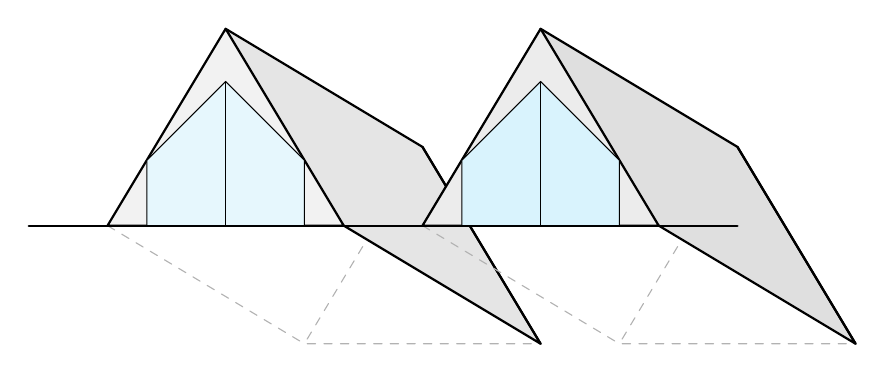
\begin{tikzpicture}[line cap=round, line join=round, >=stealth, font=\footnotesize, scale=1]
			
			% Dùng hệ trục tọa độ 3D tùy biến để vẽ hai ngôi nhà song song (Cavalier Projection)
			\tikzset{
				3dview/.style={
					x={(1cm,0cm)},
					y={(0.5cm,-0.3cm)},
					z={(0cm,1cm)}
				}
			}
			
			\begin{scope}[3dview]
				% ----------------------------------------------------
				% NGÔI NHÀ THỨ NHẤT (Bên trái / Phía sau)
				% ----------------------------------------------------
				
				% Tọa độ các đỉnh của Nhà 1 (Gốc tại O)
				\coordinate (A1) at (0,0,0);
				\coordinate (B1) at (3,0,0);
				\coordinate (C1) at (3,5,0);
				\coordinate (D1) at (0,5,0);
				\coordinate (S1) at (1.5,0,2.5); % Đỉnh mái trước
				\coordinate (E1) at (1.5,5,2.5); % Đỉnh mái sau
				
				% Vẽ các đường khuất của Nhà 1
				\draw[dashed, gray!60, thin] (A1)--(D1)--(C1);
				\draw[dashed, gray!60, thin] (E1)--(D1);
				
				% Tô màu các mặt thấy được của Nhà 1
				\fill[gray!10] (A1)--(B1)--(S1)--cycle; % Mặt trước
				\fill[gray!20] (B1)--(C1)--(E1)--(S1)--cycle; % Mái phải
				
				% Vẽ các cạnh thấy được của Nhà 1
				\draw[thick] (A1)--(B1)--(S1)--cycle;
				\draw[thick] (B1)--(C1)--(E1)--(S1);
				\draw[thick] (C1)--(E1);
				
				% Chi tiết cửa của Nhà 1 (Cửa kính lớn mặt trước)
				\draw[thin, fill=cyan!10] (0.5,0,0) -- (0.5,0,0.83) -- (1.5,0,1.83) -- (2.5,0,0.83) -- (2.5,0,0) -- cycle;
				\draw[thin] (1.5,0,0) -- (1.5,0,1.83); % Khung dọc cửa
				
				% ----------------------------------------------------
				% NGÔI NHÀ THỨ HAI (Bên phải / Phía trước - Tịnh tiến theo trục X)
				% ----------------------------------------------------
				\def\dx{4} % Khoảng cách giữa hai nhà theo trục X
				
				\coordinate (A2) at (0+\dx,0,0);
				\coordinate (B2) at (3+\dx,0,0);
				\coordinate (C2) at (3+\dx,5,0);
				\coordinate (D2) at (0+\dx,5,0);
				\coordinate (S2) at (1.5+\dx,0,2.5);
				\coordinate (E2) at (1.5+\dx,5,2.5);
				
				% Vẽ các đường khuất của Nhà 2
				\draw[dashed, gray!60, thin] (A2)--(D2)--(C2);
				\draw[dashed, gray!60, thin] (E2)--(D2);
				
				% Tô màu các mặt thấy được của Nhà 2
				\fill[gray!15] (A2)--(B2)--(S2)--cycle;
				\fill[gray!25] (B2)--(C2)--(E2)--(S2)--cycle;
				
				% Vẽ các cạnh thấy được của Nhà 2
				\draw[thick] (A2)--(B2)--(S2)--cycle;
				\draw[thick] (B2)--(C2)--(E2)--(S2);
				\draw[thick] (C2)--(E2);
				
				% Chi tiết cửa của Nhà 2
				\draw[thin, fill=cyan!15] (0.5+\dx,0,0) -- (0.5+\dx,0,0.83) -- (1.5+\dx,0,1.83) -- (2.5+\dx,0,0.83) -- (2.5+\dx,0,0) -- cycle;
				\draw[thin] (1.5+\dx,0,0) -- (1.5+\dx,0,1.83);
				
				% ----------------------------------------------------
				% CẢNH QUAN XUNG QUANH (Tùy chọn để tạo nền)
				% ----------------------------------------------------
				% Đường nền đất sàn trước hai nhà
				\draw[black, thick] (-1,0,0) -- (8,0,0);
				
			\end{scope}
		\end{tikzpicture}
		\begin{tikzpicture}[line cap=round, line join=round, font=\footnotesize, >=stealth, scale=0.8]
			\coordinate (O) at (0,0);
			\coordinate (y) at (-15:6);
			\coordinate (x) at (-140:4);
			\coordinate (A) at (-140:3);
			\coordinate (O') at (-15:5);
			\coordinate (z) at (90:4);
			\coordinate (C) at (90:2);
			\coordinate (B) at (-1,3);
			\coordinate (A') at ($(A)+(O')-(O)$);
			\coordinate (B') at ($(A')+(B)-(A)$);
			\coordinate (I) at 	(intersection of O--z and B'--B);
			\draw[->](A)--(x);
			\draw[->](O')--(y);
			\draw[->](I)--(z);
			\foreach \i/\j in {O/A,O/I,O/B,O/O'}{\draw[dashed](\i)--(\j);}
			\draw (B')--(O')--(A');
			\draw (A)--(B)--(B')--(A')--cycle;
			\foreach \i/\g in {O/180,A/180,B/90,A'/-30,B'/90,O'/60}{\draw[fill=black](\i) circle (1pt) ($(\i)+(\g:3mm)$) node[scale=1]{$\i$};}
			\foreach \i/\g in {x/-90,y/0,z/180}{\draw[fill=black]($(\i)+(\g:3mm)$) node[scale=1]{$\i$};}
		\end{tikzpicture}
	\end{center}
		\shortans[]{$26{,}8$}
		\loigiai{
			Theo hệ trục tọa độ, ta có\\
		$O(0;0;0)$, $O'(0;450;0)$, $A(240;0;0)$, $A'(240;450;0)$, $B(120;0;300)$, $B'(120;450;300)$.\\
		Vì đơn vị đo là centimet nên
		$OA=240\,\text{cm}=2,4\,\text{m}$, $OO'=450\,\text{cm}=4,5\,\text{m}$.\\
		Diện tích nền nhà là
		$S_{\text{nền}}=OA\cdot OO'=2,4\cdot4,5=10,8\,\text{m}^2$.\\
		Ta có
		$$OB=\sqrt{120^2+300^2}=\sqrt{104400}\,\text{cm}=\dfrac{\sqrt{104400}}{100}\,\text{m}.$$
		Do đó diện tích hai mái nhà là
		$$S_{\text{mái}}=2\cdot OB\cdot OO'
		=2\cdot\dfrac{\sqrt{104400}}{100}\cdot4,5
		\approx29,1\,\text{m}^2.$$
		Diện tích một mặt trước là
		$$S_{\triangle OAB}=\dfrac{1}{2}\cdot240\cdot300=36000\,\text{cm}^2=3,6\,\text{m}^2.$$
		Vậy diện tích mặt trước và mặt sau là
		$$S_{\text{trước sau}}=2\cdot3,6=7,2\,\text{m}^2.$$
		Tổng chi phí là
		$10,8\cdot200000+29,1\cdot700000+7,2\cdot600000
		=26850000$ đồng.\\
		Suy ra tổng chi phí xấp xỉ $26,8$ triệu đồng.
		}
	\end{ex}
	
	%%==========Câu 6
	\begin{ex}%[40-26-2-CaMau-SoGD-L1]%[Doan Thinh,26-2-DuAnDeTHPT2025-2026]%[0D0V2-4]
		Một trường THPT X có $12$ học sinh đạt giải học sinh giỏi cấp tỉnh năm $2026$. Trong đó học sinh giỏi môn Toán có $3$ nữ và $5$ nam, học sinh giỏi môn Vật lý thì có $4$ nam. Lãnh đạo trường chọn ngẫu nhiên ra $3$ học sinh để dự lễ tuyên dương. Tính xác suất để chọn ra được $3$ học sinh có đủ hai môn Toán và Vật lý đồng thời phải có học sinh nam và học sinh nữ? \textit{(kết quả làm tròn đến hàng phần trăm)}.
		\shortans[]{$0{,}41$}
		\loigiai{
			Gọi $A$ là biến cố \lq \lq Chọn được 3 học sinh đủ hai môn Toán và Vật lý đồng thời có học sinh nam và học sinh nữ\rq\rq.\\
			Số phần tử không gian mẫu: $n(\Omega)=\mathrm{C}_{12}^3$.\\
			\textbf{Trường hợp 1:} Chọn $1$ học sinh nữ có $\mathrm{C}_3^1$ cách.\\ 
			Khi đó:\\
			- Chọn $1$ học sinh nam môn Toán và $1$ nam môn Vật lý có $\mathrm{C}_5^1\cdot\mathrm{C}_4^1$ cách.\\
			- Chọn $2$ học sinh nam môn Vật lý có $\mathrm{C}_4^2$ cách.\\
			Trường hợp này có $\mathrm{C}_3^1\left(\mathrm{C}_5^1\cdot\mathrm{C}_4^1+\mathrm{C}_4^2\right)$ cách chọn.\\
			\textbf{Trường hợp 2:} Chọn $2$ học sinh nữ có $\mathrm{C}_3^2$ cách chọn.\\ 
			Khi đó chọn thêm $1$ học sinh nam môn Vật lý có $\mathrm{C}_4^1$ cách.\\ 
			Trường hợp này có $\mathrm{C}_3^2\cdot\mathrm{C}_4^1$ cách chọn.\\
			Vậy $ n(A)=\mathrm{C}_3^1(\mathrm{C}_5^1\cdot\mathrm{C}_4^1+\mathrm{C}_4^2)+\mathrm{C}_3^2\cdot\mathrm{C}_4^1=90$ cách chọn.\\
			Vậy xác suất cần tìm là $P(A)=\dfrac{n(A)}{n(\Omega)}=\dfrac{90}{220}\approx 0{,}41$.
		}	
	\end{ex}
\Closesolutionfile{ans}

\indapan{6}{ans/ans-26-2-CaMau-SoGD-L1-LC}
\indapan{2}{ans/ans-26-2-CaMau-SoGD-L1-DS}
\indapan{6}{ans/ans-26-2-CaMau-SoGD-L1-KQ}



